\documentclass[a4paper,12pt]{article}

\usepackage[utf8]{inputenc}
\usepackage[T1]{fontenc}
%\usepackage[french]{babel}
\usepackage[margin=2cm]{geometry}
\usepackage{graphicx}
\usepackage{textcomp}
\usepackage{verbatim}
\usepackage{pdfpages}
\usepackage{url}
\usepackage{hyperref}
\usepackage{tabto}
\usepackage{mathtools, bm}
\usepackage{amssymb, bm}
\usepackage{dsfont}
\usepackage{amsmath, amsfonts, amssymb}

\hypersetup{linktoc=all}

\newcommand{\ts}{\textsuperscript}
\newcommand{\tr}{\textregistered}

\begin{document}


	%frontmatter
		\begin{titlepage}
	\begin{center}
		\vspace*{2.5cm}
		\textbf{
		\huge{
		\textsc{Rapport du projet}\\}}

		\vspace{5cm}

		\LARGE{
		\textsc{Navier-Stokes 2D en C++}\\[0.5\baselineskip]
		Thibault Cimic\\

		\vspace{5cm}
		\textsc{\today}\\ 

		\vspace{1cm}
		\textsc{Superviseur:\\
		F. Hecht}\\

		\vspace{1cm}
		\textsc{Paris\\
		Universite Pierre et Marie Curie}\\}

		\end{center}

\end{titlepage}
		%\tableofcontents
 	  \setcounter{page}{1}
		
Dans ce projet, nous tentons d'implémenter un code C++ qui modélise l'écoulement d'un fluide sur un maillage 2D. Pour cela, nous tentons de faire un solveur éléments finis pour les équations de Navier-Stokes.
La méthode est alors premièrement de faire un solveur pour les équations de Stokes, ce qui correspond à modéliser les équations de Navier-Stokes sous l'hypothèse que notre fluide est de densité volumique très faible, mais toujours incompressible.
Nous verrons donc en première partie la gestion du problème pour les équations de Stokes, puis le passage aux équations de Navier-Stokes générales, et enfin l'application au domaine de la marche.

Pour modéliser ce fluide, nous implémentons une méthode d'éléments finis $\mathbb{P}^{2}$-Lagrange pour la vitesse, et $\mathbb{P}^1$-Lagrange pour la pression, et on gère la non-linéarité des équations de Navier-Stokes par la méthode des caractéristiques rétrograde.

\newpage
		
\section{Le problème de Stokes}

\subsection{Le cadre théorique}

Soit $\Omega \subset \mathbb{R}^{2}$ un polyhèdre. Les équations de Stokes qui nous intéressent s'écrivent sous la forme :

\begin{equation}
\left \{
\begin{array}{c @{ = } c}
    -\nu \Delta u + \nabla p \text{ } & f \text{ in } \Omega\\
    \nabla . u & \text{ } 0 \text{ in } \Omega\\
    u & \text{ } 0 \text{ on } \partial\Omega \backslash \Gamma\\
    \nu\partial_{n}u - pn & 0 \text{ on } \Gamma\\
\end{array}
\right.
\end{equation}

où $u = (u_{1},u_{2})^{t} : \Omega \mapsto \mathbb{R}^{2}$ est le champ de vitesse dans $H^{1}\left(\Omega\right)^{2}$, $p : \Omega \mapsto \mathbb{R}$ est la pression dans $L^{2}_{*}\left(\Omega\right) = \left \{ q \in L^{2}\left( \Omega \right) | \int_{\Omega} q = 0 \right \}$, $f = (f_{1},f_{2})^{t} : \Omega \mapsto \mathbb{R}^{2}$ est un second membre quelconque dans $L^{2}\left( \Omega \right)^{2}$, $\nu$ est la viscosité du fluide, et enfin $n$ est le normale extérieur unitaire à $\Omega$.

Pour cette partie, si l'on désire plus de détails, on peut consulter la référence [1], le livre Mathematical Aspects of Discontinuous Galerkin Methods, de A. Ern et D. A. Di Pietro, chap. 6.


\subsection{Formulation variationnelle et système linéaire}

On pose :
\begin{equation}
U := H^{1}_{\partial \Omega \backslash \Gamma, 0}\left(\Omega\right)^{2} \text{, } P := L^{2}_{*}\left(\Omega\right) \text{, } X := U \times P
\end{equation}

Les espaces $U$, $P$, et $X$ sont alors des espaces de Hilbert pour les produits scalaires associés aux normes :
\begin{equation}
||v||_{U} := ||v||_{H^{1}\left(\Omega\right)^{2}} = \left( ||v_{1}||_{H^{1}\left(\Omega\right)}^{2}+||v_{2}||_{H^{1}\left(\Omega\right)}^{2} \right)^{\frac{1}{2}}
\end{equation}
\begin{equation}
||q||_{P} := ||q||_{L^{2}\left(\Omega\right)} \text{, } ||\left(v,q\right)||_{X} : = \left( ||u||_{U}^{2}+||q||_{P}^{2} \right)^{\frac{1}{2}}
\end{equation}

On définit ensuite pour tout $u,v \in U$ et pour tout $q \in P$, les formes bilinéaires :

\begin{equation}
a(u,v) := \int_{\Omega} \nabla u : \nabla v = \int_{\Omega} \nabla u_{1} . \nabla v_{1} + \nabla u_{2} . \nabla v_{2}
\end{equation}
\begin{equation}
 b(v,q) := -\int_{\Omega} q \nabla . v = - \int_{\Omega} q \frac{\partial v_{1}}{\partial x_{1}} - \int_{\Omega} q \frac{\partial v_{2}}{\partial x_{2}}
\end{equation}


Et la formulation variationnelle du problème de Stokes est alors :

\begin{equation}
\left \{
\begin{array}{c @{} c}
\text{Trouver } (u,p) \in X \text{ tels que : } \\
\nu a(u,v) + b(v,p) = \int_{\Omega} fv \text{, } \forall v \in U \\
-b(u,q) = 0 \text{, } \forall q \in P\\
\end{array}
\right.
\end{equation}

Soit $h > 0$ le paramètre d'un maillage $\mathcal{T}_{h}$, composé de $N_{s}$ sommets, $N_{t}$ triangles, et $N_{a}$ arêtes. Pour établir la formulation variationnelle discrète, il nous faut définir les espaces variationnels discrets :

\begin{equation}
U_{h} := \mathbb{P}^{2} \left( \mathcal{T}_{h} \right)^{2} = \left \{ v \in C^{0}\left( \overline{\Omega} \right) | \forall T \in \mathcal{T}_{h}, v_{|T} \in \mathbb{P}^{2}\left( T \right) \right \}^{2}
\end{equation}
\begin{equation}
P_{h} := \mathbb{P}^{1} \left( \mathcal{T}_{h} \right) = \left \{  q \in C^{0} \left( \overline{\Omega} \right) | \forall T \in \mathcal{T}_{h}, q_{|T} \in \mathbb{P}^{1}\left( T \right)  \right \}
\end{equation}

Une base de $\mathbb{P}^{1} \left( \mathcal{T}_{h} \right)$ est alors l'ensemble des fonctions qui valent 1 en un sommet du maillage et 0 sur tous les autres sommets et qui sont affines sur les triangles.\\
On a donc que : $dim(\mathbb{P}^{1} \left( \mathcal{T}_{h} \right))=N_{s} =: N^{P1}$ et on note $\left( \psi_{j} \right)_{0 \leq j \leq N^{P1}-1}$ une base de cette espace.

Une base de $\mathbb{P}^{2} \left( \mathcal{T}_{h} \right)$ est l'ensemble des fonctions qui valent 1 soit en un sommet du maillage, soit au milieu d'une arête et qui vaut 0 sur tout les autres sommets et tout les autres milieux d'arêtes et qui sont des polynômes de degré 2 sur les triangles.\\
On a donc que : $dim(\mathbb{P}^{2} \left( \mathcal{T}_{h} \right)) = N_{s}+N_{a} =: N^{P2}$ et on note $\left( \varphi_{j} \right)_{0 \leq j \leq N^{P2}-1}$ une base de cette espace.

On a donc les équivalences suivantes qui nous amène de la formulation variationnelle discrète au système linéaire :
\begin{equation}
\left \{
\begin{array}{c @{} c}
\text{Trouver } (u_{h},p_{h}) \in X_{h} \text{ tels que : } \\
\nu a(u_{h},v_{h}) + b(v_{h},p_{h}) = \int_{\Omega} fv_{h} \text{, } \forall v_{h} \in U_{h} \\
-b(u_{h},q_{h}) = 0 \text{, } \forall q_{h} \in P_{h}\\
\end{array}
\right.
\end{equation}
\begin{equation}
\iff \left \{
\begin{array}{c @{} c}
\text{Trouver } (u_{h},p_{h}) \in X_{h} \text{ tels que : } \\
\nu \int_{\Omega} \nabla u_{h}^{1} . \nabla \varphi_{j}^{1} + \nabla u_{h}^{2} . \nabla \varphi_{j}^{2} - \int_{\Omega} p_{h} \frac{\partial \varphi_{j}^{1}}{\partial x_{1}} - \int_{\Omega} p_{h} \frac{\partial \varphi_{j}^{2}}{\partial x_{2}} = \int_{\Omega} f \varphi_{j}^{1} + f\varphi_{j}^{2}, \; \forall 0 \leq j \leq N^{P2}-1\\
\int_{\Omega} \psi_{j} \frac{\partial u_{h}^{1}}{\partial x_{1}} + \psi_{j} \frac{\partial u_{h}^{2}}{\partial x_{2}} = 0, \; \forall 0 \leq j \leq N^{P1}-1
\end{array}
\right.
\end{equation}
On écrit ensuite $u_{h}^{1}$, $u_{h}^{2}$, et $p_h$ dans les bases des espaces variationnels :
\begin{equation}
u_{h}^{l} = \sum_{j=0}^{N^{P2}-1} u_{h,j}^{l} \varphi_{j}^{l}, l = 1, 2
\end{equation}
\begin{equation}
p_{h} = \sum_{j = 0}^{N^{P1}-1} p_{h,j}\psi_{j}
\end{equation}
En notant :
\begin{equation}
U = \left( \left( u_{h,j}^{1} \right)_{0 \leq j \leq N^{P2}}, \left( u_{h,j}^{2} \right)_{0 \leq j \leq N^{P2}}, \left( p_{h,j} \right)_{0 \leq j \leq N^{P1}} \right)^{t} \in \mathbb{R}^{2*N^{P2}+N^{P1}}
\end{equation}
On a :
\begin{equation}
(11) \iff \left \{
\begin{array}{c @{} c}
\text{Trouver } U \in \mathbb{R}^{2*N^{P2}+N^{P1}} \text{, tel que :} \\
\begin{pmatrix}
\nu Rig_{1} & 0 & D_{1} \\
0 & \nu Rig_{2} & D_{2} \\
D_{1}^{t} & D_{2}^{t} & 0 \\
\end{pmatrix} U = F\\
\end{array}
\right.
\end{equation}
où :
\begin{equation}
Rig_{l} = \left( \int_{\Omega} \nabla \varphi_{i}^{l} \nabla \varphi_{j}^{l} \right)_{0 \leq i,j \leq N^{P2}-1}, l = 1,2
\end{equation}
\begin{equation}
D_{l} = \left( -\int_{\Omega} \psi_{j} \frac{\partial \varphi_{i}^{l}}{\partial x_{l}} \right)_{\substack{
0 \leq i \leq N^{P2}-1 \\
0 \leq j \leq N^{P1}-1
}}, l=1,2
\end{equation}
\begin{equation}
F = \left( \left( \int_{\Omega} f\varphi_{j}^{1} \right)_{0 \leq j \leq N^{P2}-1}, \left( \int_{\Omega} f\varphi_{j}^{2} \right)_{0 \leq j \leq N^{P2}-1}, \left( 0 \right)_{0 \leq j \leq N^{P1}-1} \right)
\end{equation}

Pour cette partie, si l'on désire plus de détails, on peut consulter la référence [1], le livre Mathematical Aspects of Discontinuous Galerkin Methods, de A. Ern et D. A. Di Pietro, chap. 6.


\subsection{Implémentation}

\subsubsection{Assemblage du système linéaire}

Pour résoudre numériquement le système linéaire $(15)$, il nous faire une lègere modification sur le problème variationnel $(10)$. Cette modification consiste à rajouter un terme de masse pour la pression comme ceci :

\begin{equation}
\left \{
\begin{array}{c @{} c}
\text{Trouver } (u_{h},p_{h}) \in X_{h} \text{ tels que : } \\
\nu a(u_{h},v_{h}) + b(v_{h},p_{h}) = \int_{\Omega} fv_{h} \text{, } \forall v_{h} \in U_{h} \\
-b(u_{h},q_{h}) - \varepsilon \int_{\Omega} q_{h} p_{h} = 0 \text{, } \forall q_{h} \in P_{h}\\
\end{array}
\right.
\end{equation}

où $\varepsilon$ est un paramètre voué à être petit, au sens où il existe un résultat qui stipule que lorsque $\varepsilon \longrightarrow 0$, la solution du problème variationnel $(19)$ tend bien vers la solution du problème variationnel $(10)$.

Pour davantage sur ce résultat, on peut consulter la référence [2], Finite Element Methods for Navier-Stokes Equations, V. Girault
et P.-A. Raviart, chap. I § 4.3.

Cette modification vas alors se traduire de la manière suivante sur notre système linéaire :

\begin{equation}
(19) \iff \left \{
\begin{array}{c @{} c}
\text{Trouver } U \in \mathbb{R}^{2*N^{P2}+N^{P1}} \text{, tel que :} \\
\begin{pmatrix}
\nu Rig_{1} & 0 & D_{1} \\
0 & \nu Rig_{2} & D_{2} \\
D_{1}^{t} & D_{2}^{t} & -\varepsilon Mass \\
\end{pmatrix} U = F\\
\end{array}
\right.
\end{equation}

où tout est identique à la situation précédente, avec :

\begin{equation}
Mass = \left( \int_{\Omega} \psi_{i} \psi_{j} \right)_{0 \leq i,j \leq N^{P1}-1}
\end{equation}

Enfin, pour résoudre ce problème, il nous faut être capable de calculer les fonctions de formes $\mathbb{P}^2$ et $\mathbb{P}^1$ sur n'importe quel triangle du maillage $\mathcal{T}_{h}$.

Pour cela, on vas calculer ces fonctions de formes sur un triangle de référence puis calculer la transformation affine qui envoie ce triangle de référence sur un triangle de notre maillage.

Le triangle de référence est le triangle $\widehat{T}$ composé des trois sommets $\widehat{x}_{0} = (0,0) , \widehat{x}_{1} = (1,0) , \widehat{x}_{2} = (0,1)$.
On a alors, au vu de la définition des fonctions de formes $\mathbb{P}^{1}$, les résultats suivants :

\begin{equation}
\left \{
\begin{array}{c @{} c}
\widehat{\psi}_{0} \left( x_{1},x_{2} \right)  = 1-x_1-x_2 & \text{, } \nabla \widehat{\psi}_0 = \left( \begin{matrix}
-1 \\
-1 \\
\end{matrix} \right) \\
\widehat{\psi}_{1} \left( x_{1},x_{2} \right)  = x_1 & \text{, } \nabla \widehat{\psi}_1 = \left( \begin{matrix}
1 \\
0 \\
\end{matrix} \right) \\
\widehat{\psi}_{2} \left( x_{1},x_{2} \right)  = x_2 & \text{, } \nabla \widehat{\psi}_2 = \left( \begin{matrix}
0 \\
1 \\
\end{matrix} \right) \\
\end{array}
\right.
\end{equation}

Et du dessin suivant, on tire les expressions des fonctions de formes $\mathbb{P}^{2}$ sur $\widehat{T}$,

\begin{figure}[!t]                                                                                                                                                                                                                                                                                                                                                                                
		\centering
        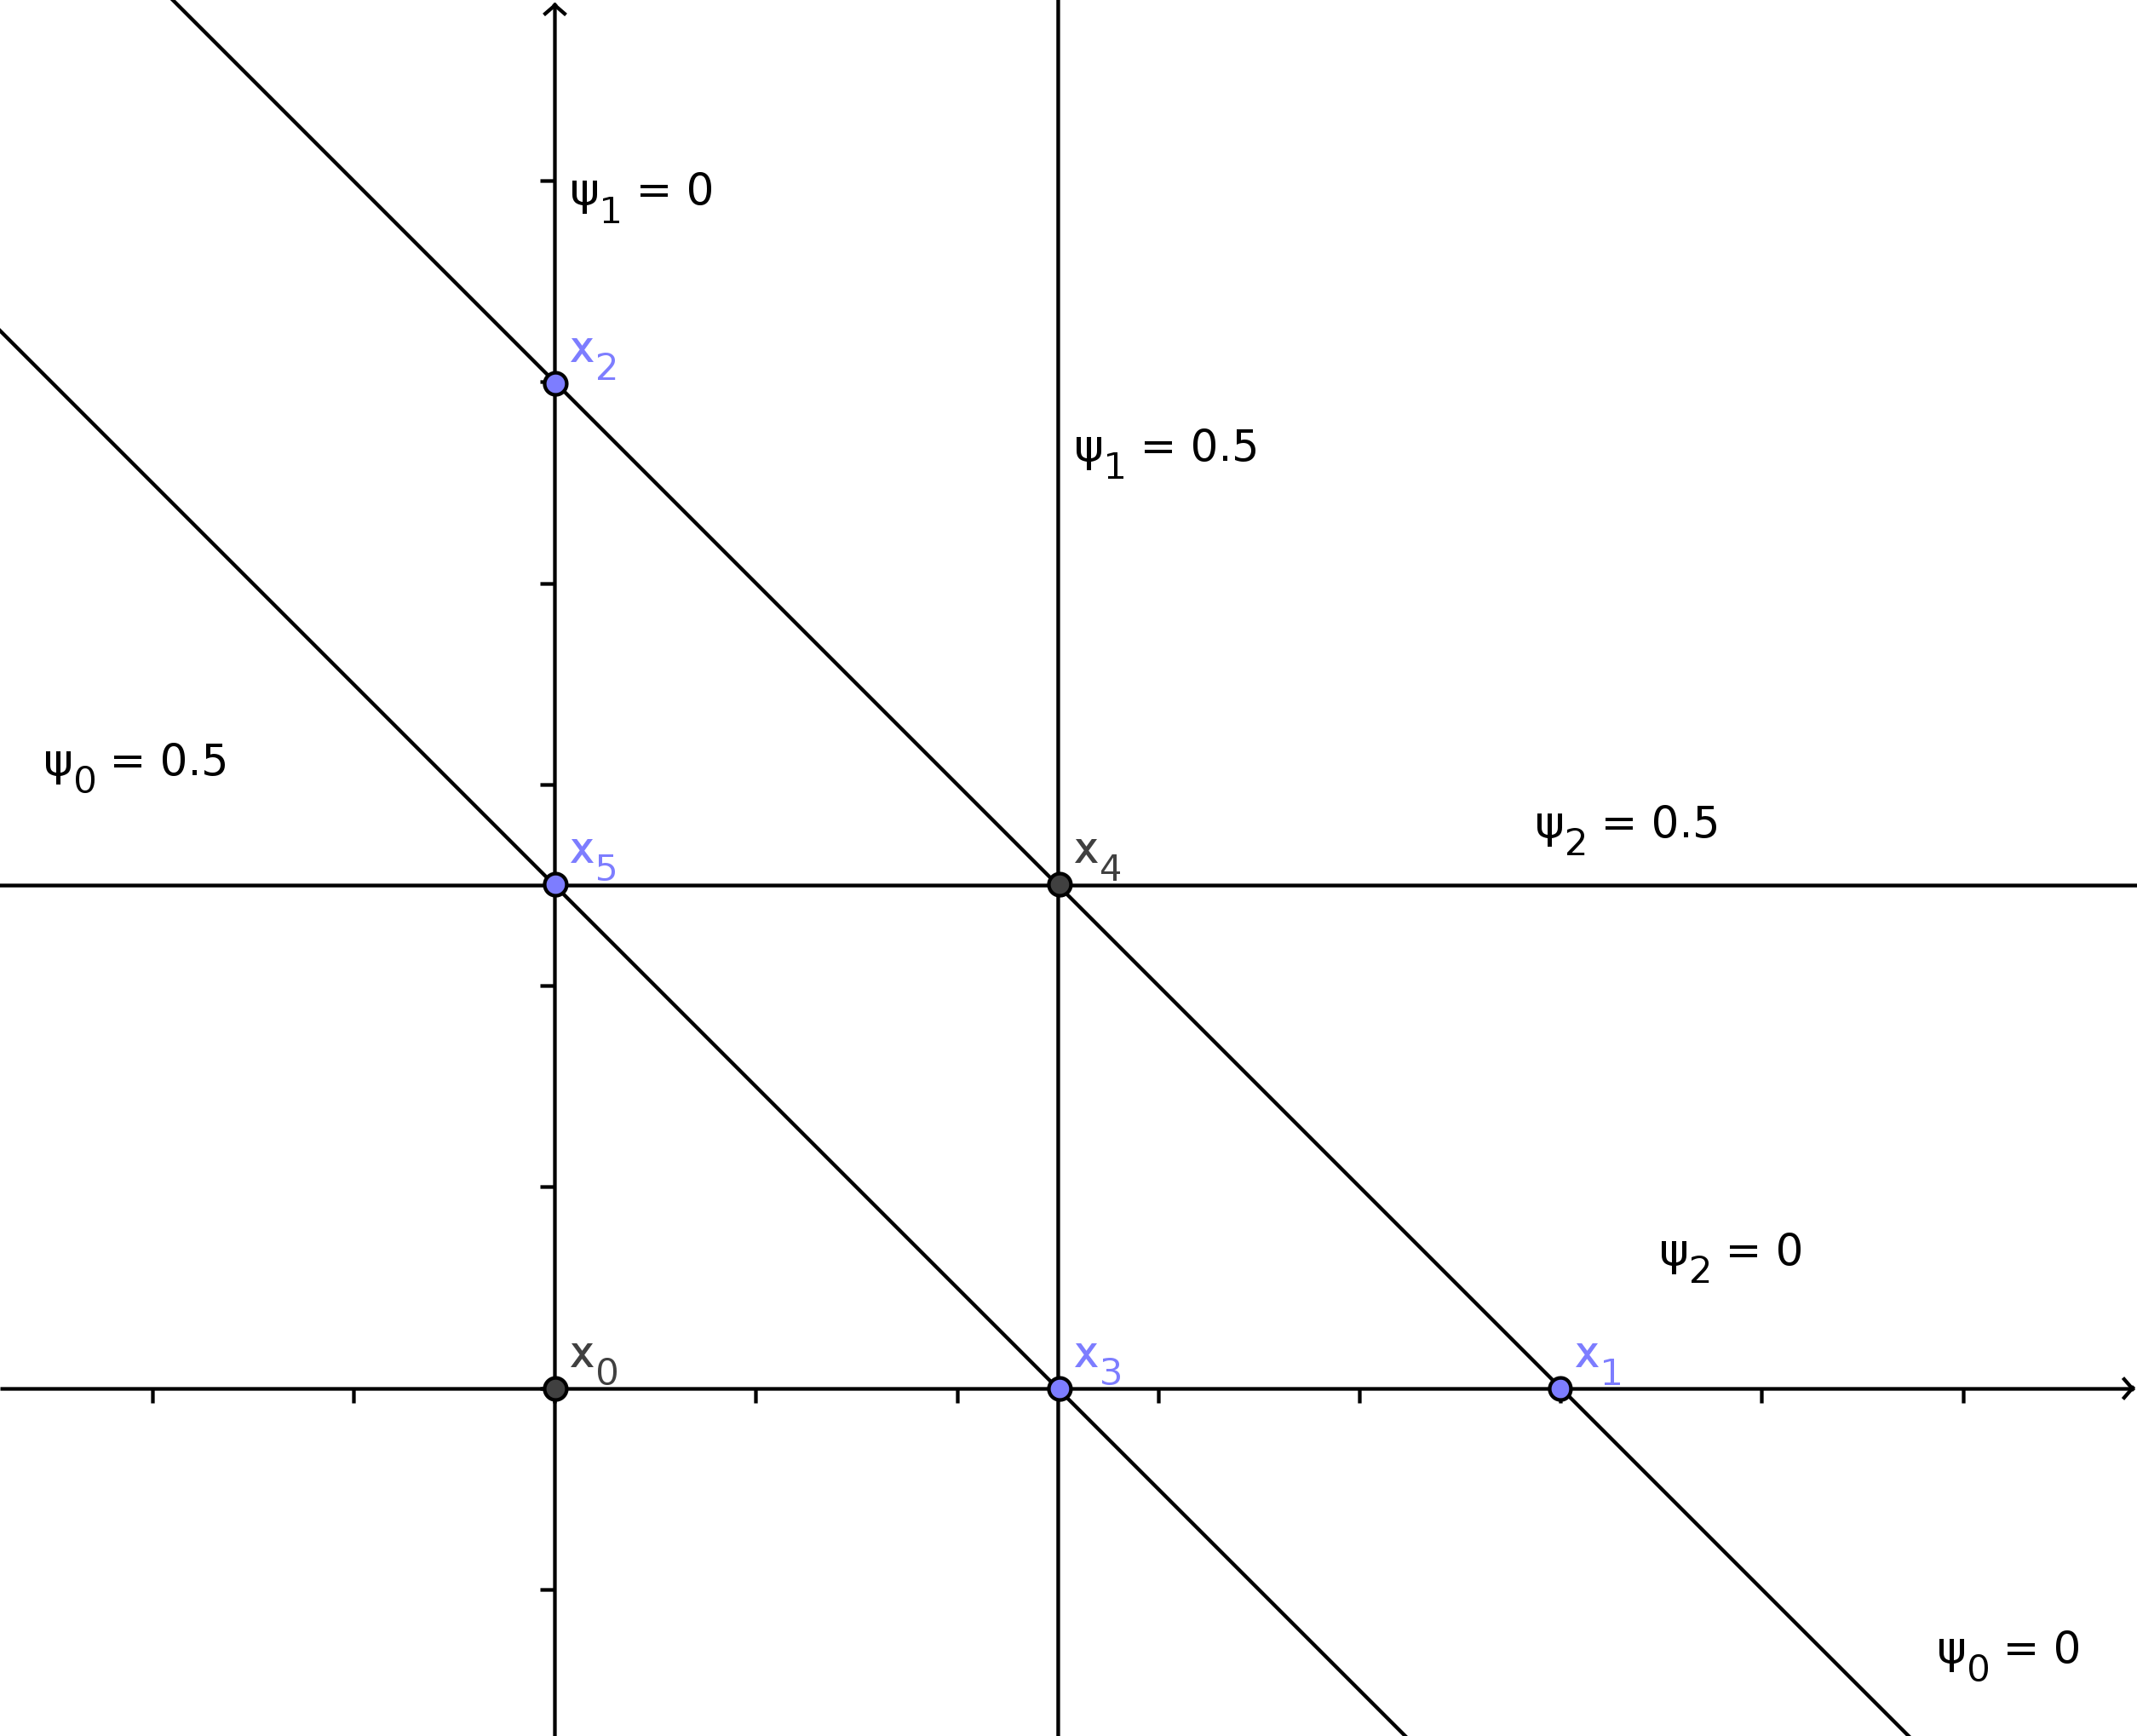
\includegraphics[width = 0.5\linewidth]{image/triang_ref}                                                                                                                                                                                                                                                                                                                                               
\caption{Triangle de référence et isovaleurs des fonctions de formes $\mathbb{P}^{1}$}                                                                                                                                        
\end{figure}

qui sont :

\begin{equation}
\left \{
\begin{array}{c @{} c}
\widehat{\varphi}_0  = \widehat{\psi}_0 \left( 2\widehat{\psi}	_0 -1 \right) & \text{, } \nabla \widehat{\varphi}_0 = 4\widehat{\psi}_0 \nabla \widehat{\psi}_0 - \nabla \widehat{\psi}_0 \\
\widehat{\varphi}_1  = \widehat{\psi}_1 \left( 2\widehat{\psi}	_1 -1 \right) & \text{, } \nabla \widehat{\varphi}_1 = 4\widehat{\psi}_1 \nabla \widehat{\psi}_1 - \nabla \widehat{\psi}_1 \\
\widehat{\varphi}_2  = \widehat{\psi}_2 \left( 2\widehat{\psi}	_2 -1 \right) & \text{, } \nabla \widehat{\varphi}_2 = 4\widehat{\psi}_2 \nabla \widehat{\psi}_2 - \nabla \widehat{\psi}_2 \\
\widehat{\varphi}_3  = 4\widehat{\psi}_0\widehat{\psi}_1 & \text{, } \nabla \widehat{\varphi}_3 = 4 \left( \nabla \widehat{\psi}_0 \widehat{\psi}_1 + \widehat{\psi}_0 \nabla \widehat{\psi}_1 \right) \\
\widehat{\varphi}_4  = 4\widehat{\psi}_1\widehat{\psi}_2 & \text{, } \nabla \widehat{\varphi}_4 = 4 \left( \nabla \widehat{\psi}_1 \widehat{\psi}_2 + \widehat{\psi}_1 \nabla \widehat{\psi}_2 \right) \\
\widehat{\varphi}_5  = 4\widehat{\psi}_2\widehat{\psi}_0 & \text{, } \nabla \widehat{\varphi}_4 = 4 \left( \nabla \widehat{\psi}_2 \widehat{\psi}_0 + \widehat{\psi}_2 \nabla \widehat{\psi}_0 \right) \\
\end{array}
\right.
\end{equation}
On dispose ainsi des fonctions formes et de leur gradient sur le triangle $\widehat{T}$. Il nous faut maintenant expliciter pour chaque triangle du maillage, la fonction affine qui envoie le triangle $\widehat{T}$ sur le triangle quelconque du maillage.

Soit donc $T \in \mathcal{T}_h$ de sommets $x_{0}, x_{1} , x_{2}$. On cherche une fonction $\mathcal{F}_{T}$ de la sorte :

\begin{equation}
\left \{
\begin{array}{c @{} c}
\mathcal{F}_{T} \left( \widehat{T} \right) = T\\
\forall \widehat{x} \in \widehat{T}, \mathcal{F}_T \left( \widehat{x} \right) = B_T \widehat{x} + a_T\\
\end{array}
\right.
\end{equation}
En particulier, on a l'équivalence suivante :
\begin{equation}
\forall i = 0,1,2, \; \mathcal{F}_T \left( \widehat{x}_i \right) = x_i \iff B_T = \left( x_1 - x_0 | x_2 -x_0 \right), \; a_T = x_0
\end{equation}
Et donc la transformation $\mathcal{F}_T$ est entièrement déterminée par les sommets de $T$.

$\mathcal{F}_T$ est alors une bijection de $\widehat{T}$ dans $T$ dès que $T$ est non-dégénéré, et on a : $|Jac \left( \mathcal{F}_T \right) | = | B_T | = \frac{|T|}{|\widehat{T}|}$.

Nous expliquons ensuite comment utiliser cela pour calculer les coefficients dans les blocs de la matrice du système linéaire $(20)$. Nous traitons ici le cas des fonctions de formes $\mathbb{P}^2$, i.e. les termes du bloc $Rig$, qui sont les plus éxotiques, les autres termes se traitent similairement mais en plus simples encore.

Soit $ 0 \leq i,j \leq N^{P2}-1 $, on veut calculer $\int_\Omega \nabla \varphi_i \nabla \varphi_j $. On commence par remarquer que les supports de $\varphi_i$ et $\varphi_j$ ne sont pas disjoints si et seulement si les nœuds $i,j$ sont commun à au moins un triangle. Ce qui a pour conséquence que notre matrice va être creuse, et par la même beaucoup plus rapide à construire que par une simple boucle imbriquée dans une autre sur le nombre de nœuds du maillage.

En effet, la stratégie se résume à boucler sur les triangles du maillage, et pour chaque triangle à calculer la matrice élémentaire $6\times6$ qui contient les contributions de chacun des $6$ nœuds du triangle les uns contre les autres, et à ensuite ré-injecter ces coefficients dans la matrice $Rig$ en regardant les numéros des 6 nœuds du triangle sur le maillage.

Il nous faut donc en réalité calculer : $\int_T \nabla \varphi_i \nabla \varphi_j$ pour $T \in \mathcal{T}_h$ et pour $i,j$ des numéros de nœuds du triangle $T$. Pour cela on utilise une formule de quadrature qui est exacte sur les polynômes de degré inférieures ou égales à 4.
On a :


\begin{equation*}
\begin{split}
\int_T \nabla \varphi_i (x) \nabla \varphi_j (x) dx & = \int_{\widehat{T}} \nabla \varphi_i \left( \mathcal{F}_T ( \widehat{x} ) \right) \nabla \varphi_j \left( \mathcal{F}_T (\widehat{x}) \right) \left| Jac \left( \mathcal{F}_T \right) \right| d \widehat{x} \\
& = \left| B_T \right| \int_{\widehat{T}} \nabla \varphi_i \left( \mathcal{F}_T ( \widehat{x} ) \right) \nabla \varphi_j \left( \mathcal{F}_T (\widehat{x}) \right) d\widehat{x} \\
& = \frac{\left| T \right|}{ | \widehat{T} |} | \widehat{T} | \sum_{k = 0}^{6} w_k  \nabla \varphi_i \left( \mathcal{F}_T ( \widehat{a}_k ) \right) \nabla \varphi_j \left( \mathcal{F}_T (\widehat{a}_k) \right) \\ 
& = | T | \sum_{k = 0}^{6} w_k  \nabla \varphi_i \left( \mathcal{F}_T ( \widehat{a}_k ) \right) \nabla \varphi_j \left( \mathcal{F}_T (\widehat{a}_k) \right) 
\end{split}
\end{equation*}
où les $(w_l)_{j =0,...,6}$ sont les poids d'intégrations associés aux $(a_l)_{l = 0,...,6}$, les points d'intégrations calculés sur le triangle de référence $\widehat{T}$. Il nous faut maintenant ramener les calculs des $\varphi_i$ sur le triangle de référence. Pour cela, on établit le lien suivant entre les fonctions de formes $\varphi_i$ sur le triangle $T$ et les $\widehat{\varphi_i}$ sur le triangle de référence $\widehat{T}$ :
\begin{equation*}
\begin{split}
\varphi_i (x) & = \widehat{\varphi_i} ( \widehat{x} ) \\
& = \widehat{\varphi_i} \left( \mathcal{F}^{-1}_T (x) \right)
\end{split}
\end{equation*}
Donc on a :
\begin{equation}
\begin{split}
\nabla \varphi_i (x) & = Jac \left( \mathcal{F}^{-1}_T \right) \nabla \widehat{\varphi_i} ( \widehat{x} ) \\
& = B^{-t}_T \nabla \widehat{\varphi_i} ( \widehat{x} ) 
\end{split}
\end{equation}

Ainsi, on reprends le calcul précédent, et on a :

\begin{equation}
\begin{split}
\int_T \nabla \varphi_i (x) \nabla \varphi_j (x) dx & = |T| \sum_{k=0}^{6} w_k B^{-t}_T \nabla \widehat{\varphi_i} (\widehat{a}_k) B^{-t}_T \nabla \widehat{\varphi_j} (\widehat{a}_k)
\end{split}
\end{equation}

Par le même genre de calcul, on a pour les blocs $D_1$, $D_2$ et $Mass$ :

\begin{equation*}
\begin{split}
& \int_T \psi_j \frac{\partial \varphi_i}{\partial x_l} = |T| \sum_{k=0}^{6} w_k \widehat{\psi_j} (\widehat{a}_l) \left( B^{-t}_T \nabla \widehat{\varphi}_j (\widehat{a}_l) \right)[l], \; \forall 0 \leq i \leq N^{P2}-1, \forall 0 \leq j \leq N^{P1}-1, l = 1,2  \\
& \int_T \psi_i (x) \psi_j (x) = |T| \sum_{k=0}^{6} w_k \widehat{\psi}_i (\widehat{a}_l) \widehat{\psi}_j (\widehat{a}_l), \; \forall 0 \leq i,j \leq N^{P1}-1
\end{split}
\end{equation*}

On a donc tout ce qu'il nous faut pour assembler le système linéaire $(20)$ et le résoudre. Seulement, on peut remarquer que dans la formulation variationnelle $(19)$, on ne traite pas les conditions aux limites du problème $(1)$. C'est que l'on vas faire maintenant directement sur notre système linéaire assemblé $(20)$.



\subsubsection{Gestion des conditions aux bords}

Dans un premier temps, on explique comment passer du problème $(1)$ avec des conditions de bords de type Dirichlet homogène sur $\partial \Omega \backslash \Gamma$ à des conditions de Dirichlet non homogène sur $\partial \Omega \backslash \Gamma$. Pour cela on regarde le nouveau problème suivant :

\begin{equation}
\left \{
\begin{array}{c @{ = } c}
    -\nu \Delta u + \nabla p \text{ } & f \text{ in } \Omega\\
    \nabla . u & \text{ } 0 \text{ in } \Omega\\
    u & \text{ } g \text{ on } \partial\Omega \backslash \Gamma\\
    \nu\partial_{n}u - pn & 0 \text{ on } \Gamma\\
\end{array}
\right.
\end{equation}

où les données sont exactement les mêmes que pour le problème $(1)$ et $g$ est une fonction donnée connue qui modélise le comportement imposé au fluide sur un bord de notre domaine.
Dès lors, si on note $u_g$ un relèvement de $u$ sur $\Omega$ pour la condition de bord sur $\partial \Omega \backslash \Gamma$, i.e. une fonction qui est nulle partout sauf sur $\partial \Omega \backslash \Gamma$ où elle vaut exactement $g$. On voit alors que $w=u-u_g$ satisfait le problème $(1)$ :

\begin{equation*}
\left \{
\begin{array}{c @{ = } c}
    -\nu \Delta w + \nabla p \text{ } & f \text{ in } \Omega\\
    \nabla . w & \text{ } 0 \text{ in } \Omega\\
    w & \text{ } 0 \text{ on } \partial\Omega \backslash \Gamma\\
    \nu\partial_{n}w - pn & 0 \text{ on } \Gamma\\
\end{array}
\right.
\end{equation*}

On a donc la formulation variationnelle pour $w$ qui est exactement $(7)$ :

\begin{equation*}
\begin{split}
& \left \{
\begin{array}{c @{} c}
\text{Trouver } (w,p) \in X \text{ tels que : } \\
\nu a(w,v) + b(v,p) = \int_{\Omega} fv \text{, } \forall v \in U \\
-b(w,q) = 0 \text{, } \forall q \in P\\
\end{array}
\right. \\
\iff & \left \{
\begin{array}{c @{} c}
\text{Trouver } (u,p) \in X \text{ tels que : } \\
\nu a(u,v) + b(v,p) = \int_{\Omega} fv + \nu a(u_g,v) \text{, } \forall v \in U \\
-b(u,q) = -b(u_g,q) \text{, } \forall q \in P\\
\end{array}
\right.
\end{split}
\end{equation*}

Ainsi, la gestion de la condition de Dirichlet non homogène sur le bord $\partial \Omega \backslash \Gamma$ se traduit par un changement de second membre dans notre système linéaire.

Pour $\varphi_j$ une fonction de forme $\mathbb{P}^2$ d'un nœud du bord $\partial \Omega \backslash \Gamma$, et $\psi_i$ une fonction de forme $\mathbb{P}^{1}$ d'un noeud du même bord, on a :

\begin{equation*}
\begin{split}
a(u_g,\varphi_j) & = \int_\Omega \nabla u_g : \nabla \varphi_j = \int_{\partial \Omega \backslash \Gamma} \nabla g : \nabla \varphi_j = \int_{e^{1}_j} \nabla g : \nabla \varphi_j + \int_{e^{2}_j} \nabla g : \nabla \varphi_j \\
-b(u_g,\psi_i) & = \int_\Omega \psi_i \nabla . u_g = \int_{\partial \Omega \backslash \Gamma} \psi_i \nabla . g = \int_{e^{1}_i} \psi_i \nabla . g + \int_{e^{2}_i} \psi_i \nabla . g
\end{split}
\end{equation*}

où $e^{1}_j, e^{2}_j$ et $e^{1}_i, e^{2}_i$  sont les deux arêtes du support de $\varphi_j$ resp. $\psi_i$ avec éventuellement $\varphi_j = 0$ sur l'une des deux si on est sur le milieu d'une arête.

Ainsi, une première stratégie serait de boucler sur les arêtes qui sont sur le bord, après les avoir judicieusement identifiées, de calculer les deux contributions des fonctions de formes et de les injecter à la bonne place du nœud concernés dans le second membre.
Un des problèmes de cette méthode, qui n'a pas de grande conséquences, est que la fonction $g$ est a priori quelconque, voir très irrégulière, et que donc lorsqu'on va vouloir calculer ces intégrales, une vrai question se pose vis à vis de la méthode de calcul. Quelle quadrature utilisée ? Quelle est alors l'erreur de l'utilisation de cette quadrature en fonction de la régularité de $g$ ? Ces questions ne sont en soi pas un problème, mais pour des raisons de simplicité, on préfère employer une autre stratégie.

On évite donc ces questions, et on implémente une méthode plus simple qui prend en compte ces contributions, la méthode Terrible Giant Value (TGV).

Cette méthode consiste à assembler son système linéaire sans se poser de questions et à le modifier après assemblage de la manière suivante. On repère en amont les nœuds du bord concernés par la condition de Dirichlet non homogène, notons les $\left( x^{\partial \Omega \backslash \Gamma}_j \right)_{0 \leq j \leq N^{\partial \Omega \backslash \Gamma} -1 }$, et on va remplacer toutes les valeurs diagonales des blocs $Rig_1$, et $Rig_2$ associées à ces nœuds par une $TGV$, par exemple $TGV = 10^{30}$, i.e. $(Rig_l)_{n_j,n_j} \longleftarrow TGV $ pour $ 0\leq j \leq N^{\partial \Omega \backslash \Gamma} -1 $. On vas également modifier le second membre en rentrant les valeurs $\left( TGV \times g \left( x^{\partial \Omega \backslash \Gamma}_j \right) \right)_{0 \leq j \leq N^{\partial \Omega \backslash \Gamma} -1 }$ à l'emplacement des noeuds $\left( x^{\partial \Omega \backslash \Gamma}_j \right)_{0 \leq j \leq N^{\partial \Omega \backslash \Gamma} -1 }$.

En résume, nous sommes désormais totalement capable de calculer la solution du problème de Stokes $(28)$.

\subsection{Résultats numériques}

On présente ici les graphs obtenu pour le problème de Stokes sur le domaine de la marche avec une viscosité $\nu = 1/100$ et $1/400$.

\begin{figure}[!h]
	\caption{Vitesse et pression $\nu = 1/100$, C++ VS FF++}
	\centering
	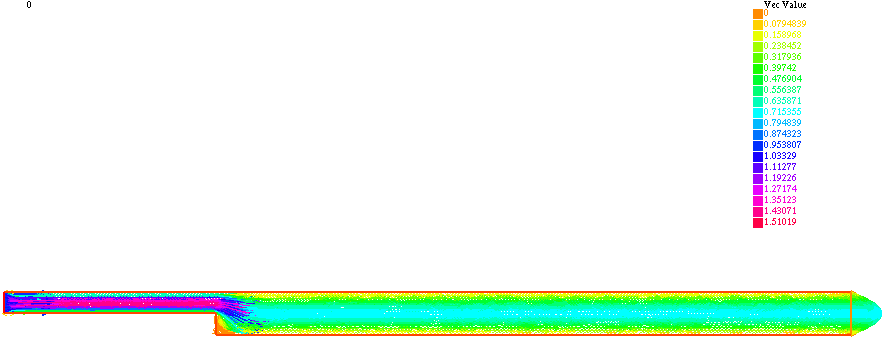
\includegraphics[width=0.49\linewidth]{image/c++_S_nu=001_t=0_u.png}
	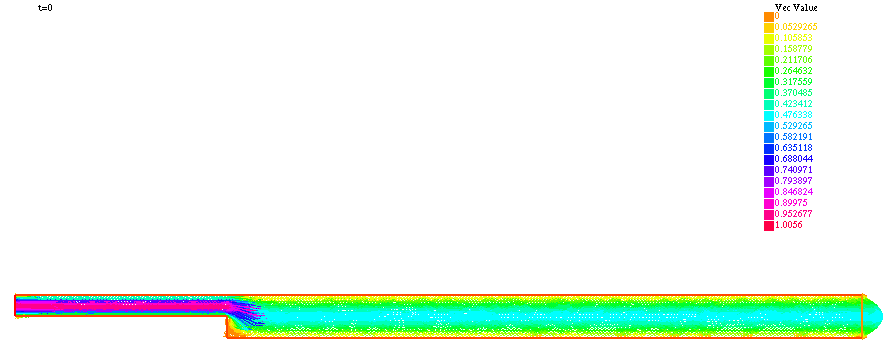
\includegraphics[width=0.49\linewidth]{image/ff++_S_nu=001_t=0_u.png}
	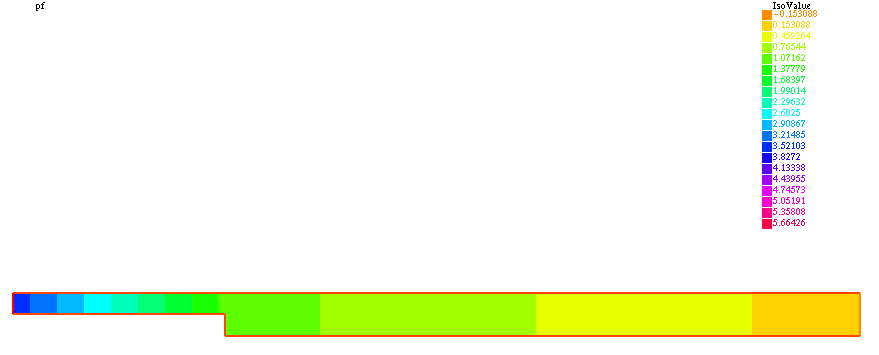
\includegraphics[width=0.49\linewidth]{image/c++_S_nu=001_t=0_p.png}
	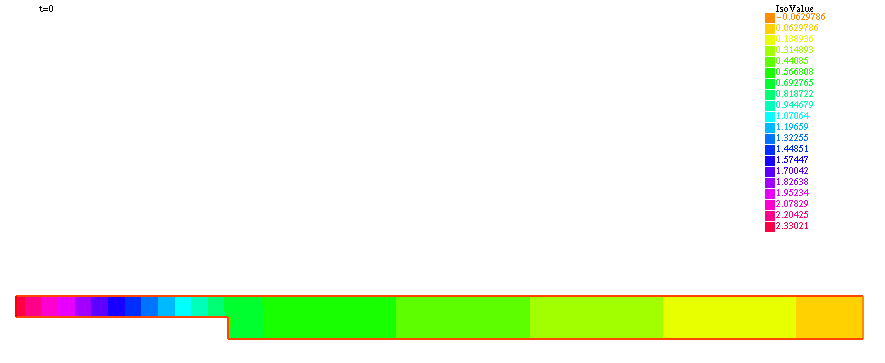
\includegraphics[width=0.49\linewidth]{image/ff++_S_nu=001_t=0_p.png}
\end{figure}

\begin{figure}[!h]
	\caption{Vitesse et pression $\nu = 1/400$, C++ VS FF++}
	\centering
	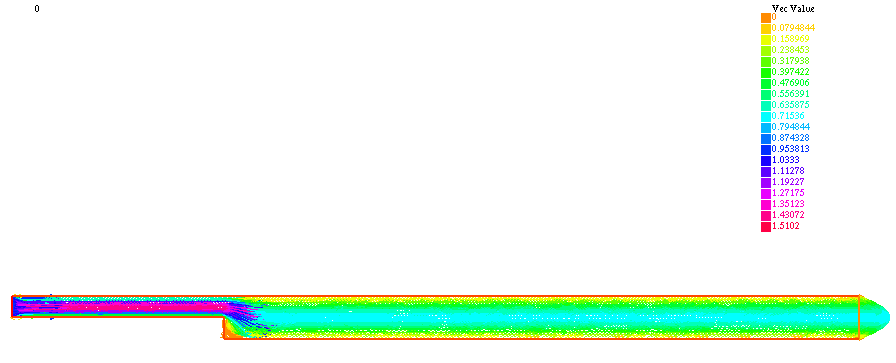
\includegraphics[width=0.49\linewidth]{image/c++_S_nu=00025_t=0_u.png}
	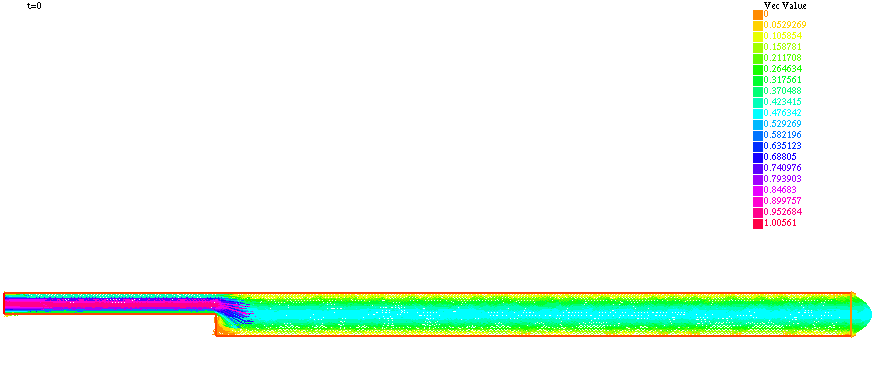
\includegraphics[width=0.49\linewidth]{image/ff++_S_nu=00025_t=0_u.png}
	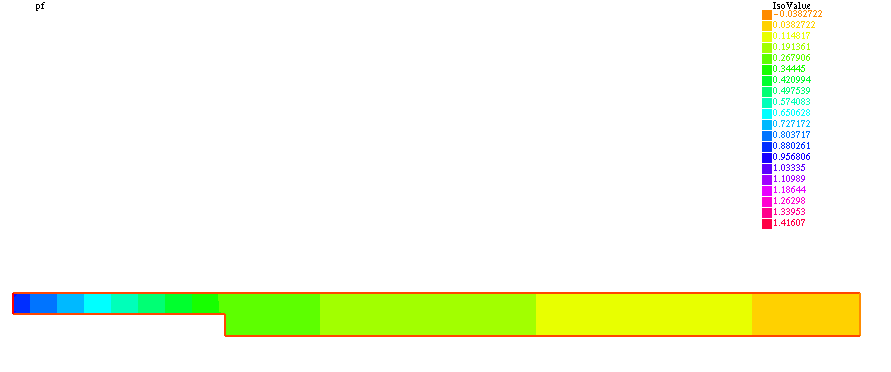
\includegraphics[width=0.49\linewidth]{image/c++_S_nu=00025_t=0_p.png}
	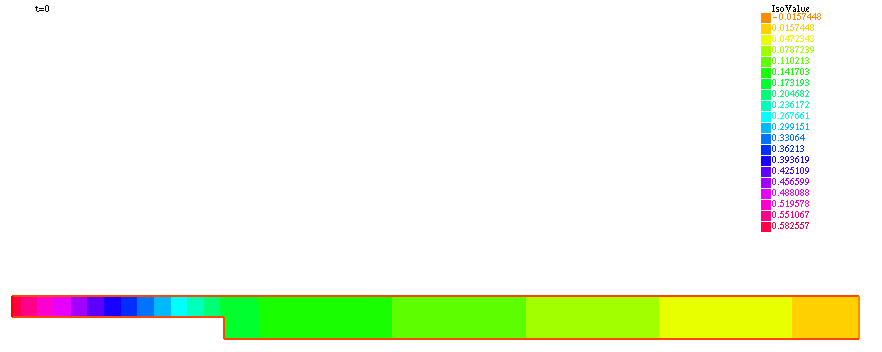
\includegraphics[width=0.49\linewidth]{image/ff++_S_nu=00025_t=0_p.png}
\end{figure}


\newpage

\section{Le problème de Navier-Stokes}


\subsection{Le cadre théorique}

Pour établir correctement le passage algorithmique des équations de Stokes à celles de Navier-Stokes, il nous faut revenir sur le formalisme mathématiques qui permet d'établir ces équations. Pour ce projet, on fait l'hypothèse que le domaine $\Omega$ est invariant en temps.

En perspective Lagrangienne, on repère une particule par le difféomorphisme suivant :

\begin{equation}
\chi (.,t,t_0) : \begin{array}{c @{} c}
\Omega \to & \Omega \\
x_0 \mapsto & x = \chi (x_0,t,t_0) 
\end{array}
\end{equation}

qui caractérise la position au temps $t$ de la particule partie de $x_0$ en $t=0$. Ainsi, la trajectoire de cette particule est la courbe $\left \{ \chi (x_0,t,t_0) \right \}_{t \in [0,T]}$, et la vitesse Lagrangienne est alors :

\begin{equation}
u(x,t) = u (\chi (x_0,t,t_0),t) = \frac{d \chi}{d t} (x_0,t,t_0)
\end{equation}

Et sous ce formalisme, le calcul de l'accélération Lagrangienne se fait par la formule dîtes formule fondamentale d'Euler pour l'accélération des fluides :

\begin{equation}
\gamma (x,t) = \frac{d u}{d t} (x,t) = \frac{\partial u}{\partial t} (x,t) + \left( u (x,t) .\nabla \right) u(x,t)
\end{equation}

Ainsi, si on considère un fluide visqueux incompressible Newtonien, de densité volumique constante en temps et en espace, on a l'équation du moment suivante issu de principe fondamentale de la dynamique :

\begin{equation}
\rho \frac{du}{dt} (x,t) = div(\sigma (x,t)) + f(x,t), \; \forall (x,t) \in \Omega \times [0,T]
\end{equation}

où $\rho$ dénote la densité volumique, $\sigma$ le tensor le tenseur des contraintes de Cauchy, et $f$ la force extérieur auquel le fluide est soumis.

Hors pour un fluide visqueux incompressible Newtonien, il se trouve que le tenseur des contraintes de Cauchy peut s'écrire sous la forme :

\begin{equation}
\sigma (x,t) = -p(x,t) Id + 2\nu D(u(x,t))
\end{equation}

où p désigne la pression, $\nu$ la viscosité, ici supposée invariante en temps et en espace, et $D(u(x,t)) = \frac{1}{2} ( \nabla u (x,t) + (\nabla u (x,t))^t )$.

Après calcul et prise en compte de la condition d'incompressibilité du fluide, on établit les équations de Navier-Stokes sous leurs formes la plus générale :

\begin{equation}
\left \{
\begin{array}{c @{} c}
\rho \left( \frac{\partial u}{\partial t}  + \left( u.\nabla \right) u \right) = -\nabla p  + \nu \Delta u  + f \\
\nabla . u  = 0 \\
\end{array}
\right.
\end{equation}

Ainsi, le terme de gauche de la première équation provient de l'accélération Lagrangienne, et le terme de droite $-\nabla p + \nu \Delta u$ provient du tenseur des contraintes de Cauchy.

On remarque que bien évidemment, lorsque $\rho$ est proche de $0$, on retrouve les équations de Stokes traitées en première partie.

La différence fondamentale entre les deux, lorsque $\rho$ n'est pas $0$, est que l'accélération Lagrangienne contient un terme non linéaire en la vitesse, $\left( u.\nabla \right) u$, ce qui complique énormément le problème d'un point de vu analyse mathématiques d'une EDP. On note, pour illustrer la difficulté du problème, que la question de l'unicité et de l'existence de solutions des équations de Navier-Stokes, pour un domaine en trois dimensions, fait encore parti à l'heure actuelle d'un des sept problèmes du prix du millénaire récompensé d'un million de dollars par l’institut Clay pour celui ou celle qui saurait y donné une démonstration ou un contre exemple.

Nous allons nous ici, gérer ce terme de non-linéarité par la méthode des caractéristiques rétrograde pour résoudre une équation de transport. C'est ce à quoi on s'attarde dans le paragraphe suivant.

\subsection{De Navier-Stokes à Stokes par la méthode des caractéristiques rétrograde}

Pour plus de simplicité, on considère que le fluide à une densité volumique constante égale à $1$, i.e. $\rho = 1$, et qu'il n'est soumis à aucune force extérieur, i.e. $f=0$. On réécrit alors les équations de Navier-Stokes sous la forme :

\begin{equation}
\left \{
\begin{array}{c @{ = } c}
 \frac{\partial u}{\partial t}  + \left( u.\nabla \right) u   -\nu \Delta u + \nabla p \; & 0 \text{ , in } \Omega \times [0,T] \\
\nabla . u  & 0 \text{ , in } \Omega \times [0,T] \\
u & \; g \text{ , on } \partial\Omega \backslash \Gamma \times [0,T] \\
\nu\partial_{n}u - pn & 0 \text{ , on } \Gamma \times [0,T] \\
u & u_0 \text{, in } \Omega \times \{0\} \\
\end{array}
\right.
\end{equation}

On va alors subdiviser l'intervalle $[0,T]$ en $N$ sous-intervalle de temps, $t_n = n \delta t$, pour $0 \leq n \leq N$, avec $\delta t = \frac{T}{N}$.

On note $u^{n+1}$ et $p^{n+1}$ les solutions de Navier-Stokes au temps $t_{n+1}$, on a :

\begin{equation}
\left \{
\begin{split}
u^{n+1} :  \begin{array}{c @{} c}
\Omega \to \mathbb{R}^2 \\
x \mapsto u(x,t_{n+1})
\end{array} \\
p^{n+1} : \begin{array}{c @{} c}
\Omega \to \mathbb{R} \\
x \mapsto p(x,t_{n+1})
\end{array}
\end{split}
\right.
\end{equation}

sont les solutions des équations de Navier-Stokes que l'on réécrit sous la forme suivante en utilisant l'accélération Lagrangienne :

\begin{equation}
\left \{
\begin{array}{c @{ = } c}
 \frac{d u^{n+1}}{d t} -\nu \Delta u^{n+1} + \nabla p^{n+1} \; & 0 \text{ , in } \Omega \times \{t_{n+1}\} \\
\nabla . u^{n+1}  & 0 \text{ , in } \Omega \times \{t_{n+1}\} \\
u^{n+1} & \; g \text{ , on } \partial\Omega \backslash \Gamma \times \{t_{n+1}\} \\
\nu\partial_{n}u^{n+1} - p^{n+1} n & 0 \text{ , on } \Gamma \times \{t_{n+1}\} \\
%u^{n+1} & u^{n+1}_{0} \text{, in } \Omega \times \{0\} \\
\end{array}
\right.
\end{equation}

On discrétise alors le terme non-linéaire caché dans l'accélération Lagrangienne en le remplaçant par un quotient différentiel d'ordre 1 :

\begin{equation}
\frac{du^{n+1}}{dt} (x_{n+1}) = \frac{u^{n+1} (x_{n+1}) - u^{n} (x_{n+1})}{\delta t} + o(\delta t)
\end{equation}

Seulement, dans le formalisme Lagrangien par lequel les équations ont été établies, la position $x_{n+1}$ de la particule de fluide dépend elle même du temps par le difféomorphisme $\chi$. En effet, on a :

\begin{equation}
u^n (x_{n+1}) = u \left( \chi (x_{n+1},t_{n+1},t_{n+1}), t_n \right)
\end{equation}

où $\chi$ est solution de l'équation de transport rétrograde suivante :

\begin{equation}
\left \{
\begin{split}
\frac{d \chi}{dt} (x_{n+1},t,t_{n+1}) = u^n \left( \chi (x_{n+1},t,t_{n+1}) \right) \\
\chi (x_{n+1},t_{n+1},t_{n+1}) = x_{n+1}
\end{split}
\right.
\end{equation}

Ce qui signifie que, le long de la caractéristique $\{ \chi (x_{n+1},t,t_{n+1}) \}_{t \in [t_n,t_{n+1}]}$, la vitesse $u^n$ est constante, et donc, on a :

\begin{equation}
u^n (x_{n+1}) = u \left( \chi (x_{n+1},t_n,t_{n+1}) , t_n \right)
\end{equation}

Il nous faut donc connaître le pied de la caractéristique au temps $t_n$, i.e. d'où est parti la particule qui est au temps $t_{n+1}$ en la position $x_{n+1}$.

Pour cela, on explicite la solution de l'équation de transport $(40)$ :

\begin{equation}
\chi (x_{n+1},t,t_{n+1}) = x_{n+1} - \int_{t}^{t_{n+1}} u^n \left( \chi (x_{n+1},s,t_{n+1}) \right) ds
\end{equation}

et comme $u^n$ est constante le long de la caractéristique $\{ \chi (x_{n+1},t,t_{n+1}) \}_{t \in [t_n,t_{n+1}]}$, on a :

\begin{equation*}
\begin{split}
\chi (x_{n+1},t_n,t_{n+1}) & = x_{n+1} - \delta t u^n \left( \chi (x_{n+1},t_{n+1},t_{n+1}) \right) \\
& = x_{n+1} - \delta t u^n ( x_{n+1} ) 
\end{split}
\end{equation*}

Donc si on sait dans quel triangle se trouve $x_{n+1}$, on peut calculer la position au temps $t_n$ de la particule qui est en $x_{n+1}$ au temps $t_{n+1}$, pour ensuite déterminer à son tour de quel triangle est parti cette particule au temps $t_n$ pour calculer $u^n (x_{n+1})$.

Ainsi, dans $(37)$ lorsqu'on remplace l'accélération Lagrangienne par le quotient différentiel dans la première équation, on obtient que $(u_{n+1},p_{n+1})$ est solution de :

\begin{equation}
\left \{
\begin{array}{c @{ = } c}
 \frac{u^{n+1} }{\delta t} -\nu \Delta u^{n+1}  + \nabla p^{n+1}  \; & \frac{u^n \circ \chi^n }{\delta t} \text{ , in } \Omega \times \{t_{n+1}\} \\
\nabla . u^{n+1}  & 0 \text{ , in } \Omega \times \{t_{n+1}\} \\
u^{n+1} & \; g \text{ , on } \partial\Omega \backslash \Gamma \times \{t_{n+1}\} \\
\nu\partial_{n}u^{n+1} - p^{n+1} n & 0 \text{ , on } \Gamma \times \{t_{n+1}\} \\
%u^{n+1} & u^{n+1}_{0} \text{, in } \Omega \times \{0\} \\
\end{array}
\right.
\end{equation}

où le second membre de la première équation est désormais complétement déterminé par la résolution de la même EDP au temps $t_n$.

Ainsi, lorsqu'on établie la formulation variationnelle de $(43)$, on retrouve la même formulation variationnelle que pour le problème de Stokes, i.e. $(7)$, à ceci près de l'ajout d'une forme bilinéaire issu de la discrétisation du terme non-linéaire de Navier-Stokes. En reprenant les mêmes notations que dans la première partie sur le problème de Stokes, on a :

\begin{equation}
\left \{
\begin{array}{c @{} c}
\text{Trouver } (u^{n+1},p^{n+1}) \in X \text{ tels que : } \\
\frac{1}{\delta t} m(u^{n+1},v) + \nu a(u^{n+1},v) + b(v,p^{n+1}) = \frac{1}{\delta t} \int_{\Omega} \left( u^n \circ \chi^n \right)  v \text{, } \forall v \in U \\
-b(u^{n+1},q) = 0 \text{, } \forall q \in P\\
\end{array}
\right.
\end{equation}

où $m$ est la forme bilinéaire définie par :

\begin{equation}
m : \begin{array}{c @{} c}
U^2 \to \mathbb{R} \\
(u,v) \mapsto \int_\Omega u v
\end{array}
\end{equation}

On va donc pouvoir traiter le problème de manière similaire qu'à la formulation variationnelle pénalisée $(19)$ :

\begin{equation}
\left \{
\begin{array}{c @{} c}
\text{Trouver } (u_{h}^{n+1},p_{h}^{n+1}) \in X_{h} \text{ tels que : } \\
\frac{1}{\delta t} m(u_{h}^{n+1},v_h) + \nu a(u_{h}^{n+1},v_{h}) + b(v_{h},p_{h}^{n+1}) = \frac{1}{\delta t}\int_{\Omega} \left( u^n \circ \chi^n \right) v_{h} \text{, } \forall v_{h} \in U_{h} \\
-b(u_{h}^{n+1},q_{h}) - \varepsilon \int_{\Omega} q_{h} p_{h}^{n+1} = 0 \text{, } \forall q_{h} \in P_{h}\\
\end{array}
\right.
\end{equation}

Et on va alors obtenir le système linéaire suivant :

\begin{equation}
(46) \iff \left \{
\begin{array}{c @{} c}
\text{Trouver } U^{n+1} \in \mathbb{R}^{2*N^{P2}+N^{P1}} \text{, tel que :} \\
\begin{pmatrix}
\frac{1}{\delta t} Mass_{1} + \nu Rig_{1} & 0 & D_{1} \\
0 & \frac{1}{\delta t} Mass_{2} + \nu Rig_{2} & D_{2} \\
D_{1}^{t} & D_{2}^{t} & -\varepsilon Mass \\
\end{pmatrix} U^{n+1} = F^{n+1} \\
\end{array}
\right.
\end{equation}

où :

\begin{equation}
U^{n+1} = \left( (u_{h,i,1}^{n+1})_{0 \leq i \leq N^{P2}-1}, (u_{h,i,2}^{n+1})_{0 \leq i \leq N^{P2}-1}, (p_{h,i}^{n+1})_{0 \leq i \leq N^{P1}-1} \right)^t
\end{equation}

et :

\begin{equation}
F^{n+1} = \left( \left( \frac{1}{\delta t} \int_\Omega \left( u^{n}_{1} \circ \chi^n \right) \varphi_i \right)_{0 \leq i \leq N^{P2}-1}, \left( \frac{1}{\delta t} \int_\Omega \left( u^{n}_{2} \circ \chi^n \right) \varphi_i \right)_{0 \leq i \leq N^{P2}-1}, \left( 0 \right)_{0 \leq j \leq N^{P1}-1} \right)
\end{equation}

avec bien évidement les matrices blocs $Mass_1$ et $Mass_2$ sont similaire à $Mass$ mais pour la dimension $N^{P2}$.

Explicitons désormais le calcul des intégrales dans le second membre. Bien évidemment, la stratégie est encore la même, on boucle sur les triangles, et on calcule les contributions de tous les noeuds $\mathbb{P}^2$ du triangle concerné que l'on injecte au bon endroit dans notre second membre. Il nous faut donc être capable de calculer, pour $T \in \mathcal{T}_h$ :

\begin{equation*}
\int_T \left( u_{l}^n \circ \chi^n \right) \varphi_i = |T| \sum_{k=0}^{6} w_k \left( u_{l}^{n} \circ \chi^n \right) (a_k) \varphi_i (a_k) = |T| \sum_{k=0}^{6} \sum_{j=0}^{5} w_k (u_{l}^{n} \circ \chi^n (a_k) )_j \varphi_j (\chi^n (a_k)) \varphi_i (a_k) 
\end{equation*}

Et grâce à une quadrature sur le triangle de référence $\widehat{T}$ que l'on ramène à notre triangle $T$ par la transformation affine $\mathcal{F}_T$, on est en mesure de calculer la position des $a_l$ dans $T$.

Seulement, comme on l'a expliqué précédemment, pour calculer $u_{l}^{n} \circ \chi^n (a_l)$, il faut savoir dans quel triangle était le point $\chi^n (a_l)$ au temps $t_n$.

Pour cela, on peut, connaissant les coordonnées de $a_l$, essayer de trouver le triangle pour lequel deux au moins de ses systèmes de coordonnées barycentriques donnent des coordonnées positives pour $\chi^n (a_l)$. La première stratégie serait alors de boucler sur la totalité des triangles et de tester deux systèmes de coordonnées barycentriques pour chaque triangle. Malheureusement, cette boucle prendrais numériquement trop de temps.

Une autre stratégie est de comprendre que l'on dispose de la vitesse en chaque triangle au temps $t_n$, et que donc si on choisit un pas de temps suffisamment petit, i.e. $0 \leq \delta t max(u^n) \leq max(h) $ où $h$ désigne par exemple la longueur de la plus grande arête du maillage, la particule d'un temps à un autre ne devrait aller que d'un triangle à un de ses voisins. Autrement dit, $a_l$ est, au temps $t_n$, dans un triangle voisin à celui dans lequel il est au temps $t_{n+1}$. Seulement, on aboutit alors à une méthode où le pas de temps est déterminer par la finesse du maillage, ce qui peut poser des problèmes pour avoir un temps de résolution acceptable.

La bonne stratégie réside dans l'idée qu'on connait les coordonnées du point recherchés : 
\begin{equation}
\chi^n (a_l) = a_l -\delta t u^n \left( a_l \right) = a_l -\delta t \sum_{j = 0}^6 u^n \left( a_l \right)_j \varphi_j \left( a_l \right)
\end{equation}

On peut donc partir du triangle $T$, regarder les voisins de $T$ et chercher si notre point est dans un triangle voisin, sinon on prends le triangle voisin à $T$ qui à le sommet qui minimise la distance à $\chi^n (a_l)$, et recommencer avec les voisins de ce triangle. On adopte ici, un stratégie légèrement différente, en effet cette méthode requiert de construire un tableau qui à un triangle associe ses triangles voisins, on a ici opté pour un tableau légèrement différents qui consiste à associer à un numéro de nœuds du maillage, tout les triangles qui partagent ce nœuds. Ainsi, au lieu de passer au triangle qui a comme le sommet qui réalise le minimum de la distance à $\chi^n (a_l)$, on passe directement à ce point et on regarde après coup, tout les triangles qui partagent ce nœuds comme sommet.

En résumé, nous avons désormais couvert toute la technicité mathématique et algorithmique nécessaires à l'implémentation du problème de Navier-Stokes. Nous allons désormais voir l'application de cette méthode à un cas particulier.

\newpage

\section{Mentions spéciales sur l'implémentation}

Nous allons dans cette partie, donner une idée des problèmes algorithmiques rencontrés lors de l'implémentation de la méthode éléments finis $\mathbb{P}^2$-$\mathbb{P}^1$ Lagrange pour le problème de Navier-Stokes.

\subsection{Les noeuds $\mathbb{P}^2$}

Pour résoudre ce problème, il faut quoiqu'il arrive générer un maillage de triangle de notre domaine, qu'on utilise un générateur de maillage ou qu'on en code un petit soi même, on se retrouve inévitablement avec un fichier de maillage qui dit quel point à quel numéro et quelles coordonnées et qui dit de quels points sont constitués les triangles. Cependant, pour faire du $\mathbb{P}^2$-Lagrange, il est nécessaire d'avoir les mêmes informations concernant les milieux des arêtes. Il nous faut donc associer un numéro à chacun des milieux des arêtes, ou de manière équivalente à chaque arête, et ce de manière unique et consistante avec la numérotation des sommets des triangles (ici, on continue juste la numérotation).
Pour ce faire, on vas parcourir les triangles et ranger les arêtes dans des classes définies par : "Deux arêtes appartiennent à la même classe si et seulement si elles ont le même plus petit numéro de sommet dont elles sont constituées."
Ainsi, pour savoir si l'on a déjà numérotée une arête, il suffit de parcourir sa classe au lieu de toutes les arêtes que l'on a déjà numérotées. Qui plus est, toutes les arêtes que l'on trouvera une deuxième fois dans l'algorithme seront exactement les arêtes à l'intérieur du maillage, et celles qu'on aura trouvées qu'une seule fois seront exactement celles qui sont sur le bord du maillage, ce qui est nécessaire de connaître pour implémenter les conditions aux bords du problème.

\subsection{L'importance du calcul différentiel}

Le bug dans ce projet que l'on a le plus de mal à débugger était un bug de calcul différentiel dans la formule $(26)$.
En effet, le calcul du jacobien de la transformation affine fait apparaître une opération de transposition de la matrice qui est dû à la manière même de calculer un jacobien. Ainsi, en ayant pas assez détaillé les calculs, cette formule est resté fausse car il n'y avait pas la transposition et cela changeait beaucoup de choses dans les coefficients de la matrice tout en ne changeant pas les propriétés "test" que peuvent présenter les matrices de masse et de rigidité.

\subsection{La sortie de maillage}

Dans le problème de Navier-Stokes, lorsque l'on assemble le second membre grâce à la méthode des caractéristiques rétrogrades, il nous faut retrouver dans quels triangles sont passés les points de quadrature qui se sont décaler par la formule $(50)$. On a déjà expliquer la stratégie à adopter, cependant il y a un problème qui n'a pas été expliqué qui se soulève lorsque précisément ces nouvelles coordonnées de points sortent du maillage. Il faut alors détecter que ce point est en dehors du maillage, et au lieu de prendre ses coordonnées on vas prendre les coordonnées du point du bord qui est le plus près, qui correspond le plus souvent à la projection orthogonale, mais pas toujours car comme notre maillage est un domaine polygonale, il y a des points du bord où la normale n'est pas définie, ou mal définie, le cas échéant il faut prendre le sommet $\mathcal{P}^1$ le plus proche.
Pour détecter qu'un point est sorti du maillage, dans notre algorithme de recherche du triangle au quel il appartient, on le sait si une fois qu'on a parcouru tout les triangles qui partagent un même point et qu'on passe au sommet qui est le plus proche on est encore au même point du maillage. Dès lors, on peut calculer le point du maillage le plus proche.

\newpage

\section{Application de la méthode sur la marche}

\subsection{Description du domaine et de son bord}

Le domaine d'étude $\Omega$ est une marche descendante de hauteur $\frac{1}{2}$ dans un canal de hauteur $1$.

\begin{figure}[h!]                                                                                                                                                                                 
\begin{center}                                                                                                                                                                                               
        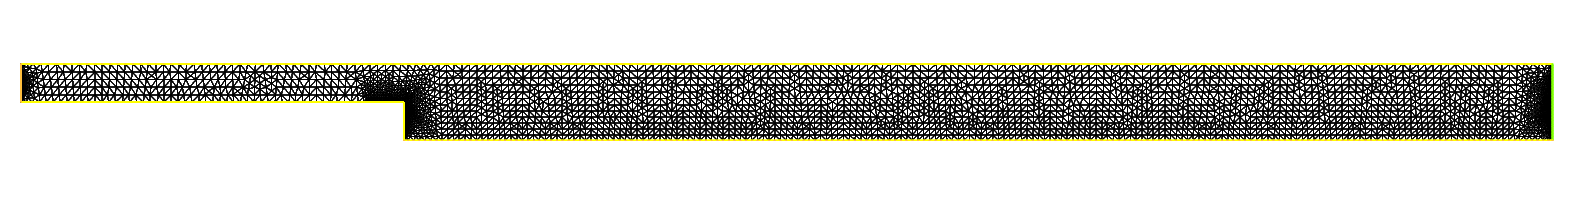
\includegraphics[scale = 0.2]{image/marche.png}                                                                                                                                              
\end{center}                                                                                                                                                                                                 
\caption{Domaine de la marche}                                                                                                                                        
\end{figure}

Vis a vis de notre problème, on y impose des conditions de Neumann sur le bord $\Gamma$ de sorti, i.e. $\nu \partial_n u - pn = 0$, une condition de Dirichlet parabolique horizontale de vitesse maximal unitaire sur le bord d'entrée, et des conditions de Dirichlet homogène sur le reste du bord. Le fluide à modéliser est régit par les équations de Navier-Stokes, avec une viscosité $\nu$, on a donc le problème suivant :

\begin{equation}
\left \{
\begin{array}{c @{ = } c}
 \frac{\partial u}{\partial t}  + \left( u.\nabla \right) u   -\nu \Delta u + \nabla p \; & 0 \text{ , in } \Omega \times [0,T] \\
\nabla . u  & 0 \text{ , in } \Omega \times [0,T] \\
u & \; u_g \text{ , on } \partial\Omega \backslash \Gamma \times [0,T] \\
\nu\partial_{n}u - pn & 0 \text{ , on } \Gamma \times [0,T] \\
u & u_0 \text{, in } \Omega \times \{0\} \\
\end{array}
\right.
\end{equation}

où :

\begin{equation}
u_g : \begin{array}{c @{} c}
\partial \Omega \backslash \Gamma \times [0,T] & \longrightarrow \mathbb{R}^2 \\
(x,t) & \mapsto \left( \begin{array}{c @{} c}
g(x_1,x_2) \\
0
\end{array}
\right)
\end{array}
\end{equation}

avec :

\begin{equation}
g : \begin{array}{c @{} c}
\partial \Omega \backslash \Gamma \to \mathbb{R} \\
(x_1,x_2) \mapsto -16(x_2-1)(x_2-\frac{1}{2}) \mathds{1}_{\{x_1 = 0\}}
\end{array}
\end{equation}

\subsection{Le cas qui fonctionne assez bien}

Pour une viscosité $\nu = 1$, on obtient avec le code C++ un résultat très similaire pour la vitesse à celui de FreeFem++ bien que les valeurs extrémales ne soient pas les mêmes, les pressions devraient ne différées que d'une constante mais ce n'est pas le cas car FreeFem++ calcule la pression de manière différente de notre code C++.
On obtient les graphs suivant :

\newpage

\begin{figure}[!t]
	\caption{Vitesse et pression $\nu = 1,t=0$, C++ VS FF++}
	\centering
	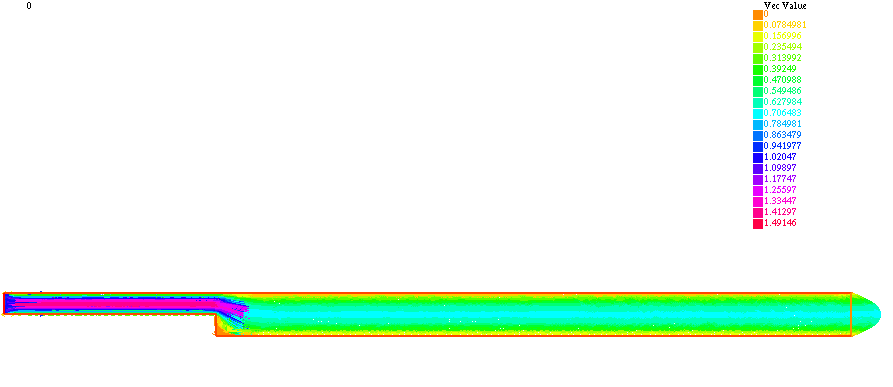
\includegraphics[width=0.49\linewidth]{image/c++_NS_nu=1_t=0_u.png}
	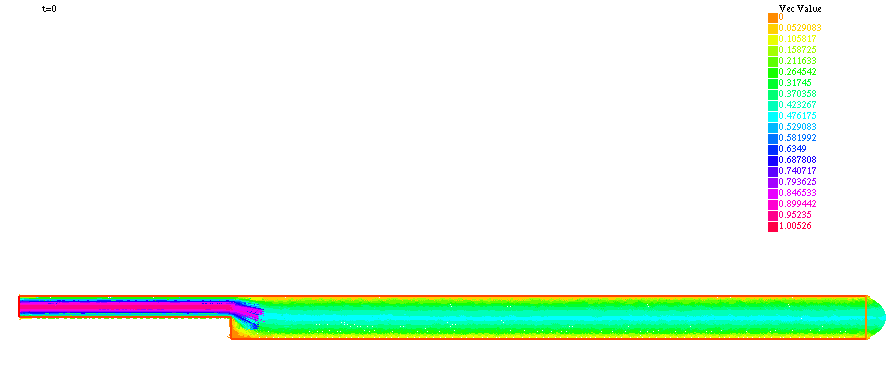
\includegraphics[width=0.49\linewidth]{image/ff++_NS_nu=1_t=0_u.png}
	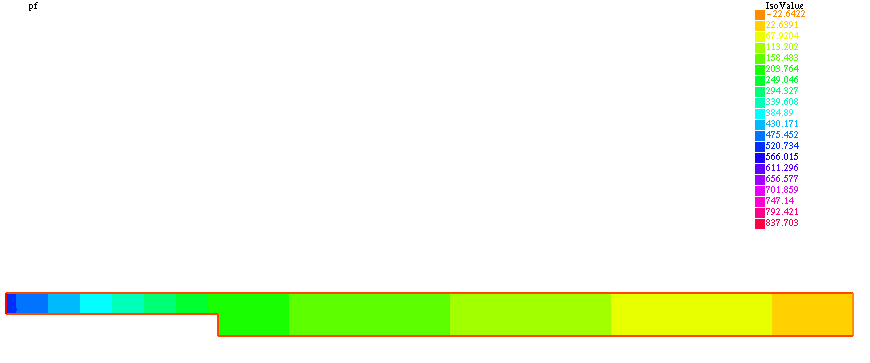
\includegraphics[width=0.49\linewidth]{image/c++_NS_nu=1_t=0_p.png}
	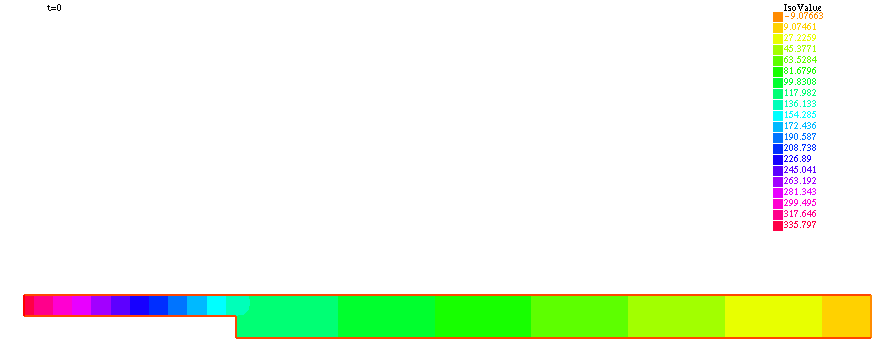
\includegraphics[width=0.49\linewidth]{image/ff++_NS_nu=1_t=0_p.png}
\end{figure}

\begin{figure}[!t]
	\caption{Vitesse et pression $\nu = 1,t=0.1$, C++ VS FF++}
	\centering
	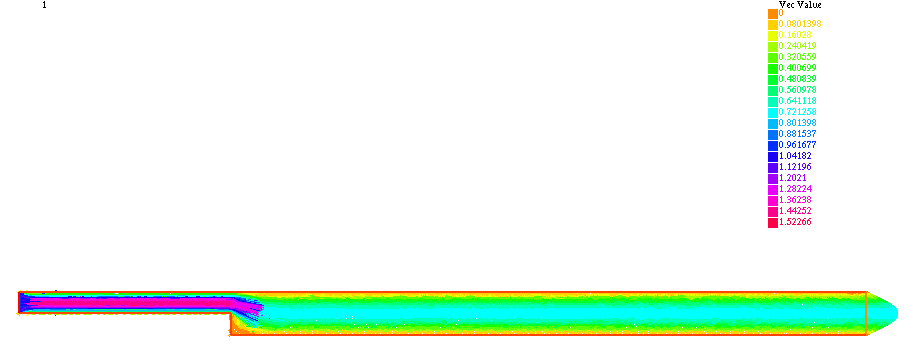
\includegraphics[width=0.49\linewidth]{image/c++_NS_nu=1_t=1_u.png}
	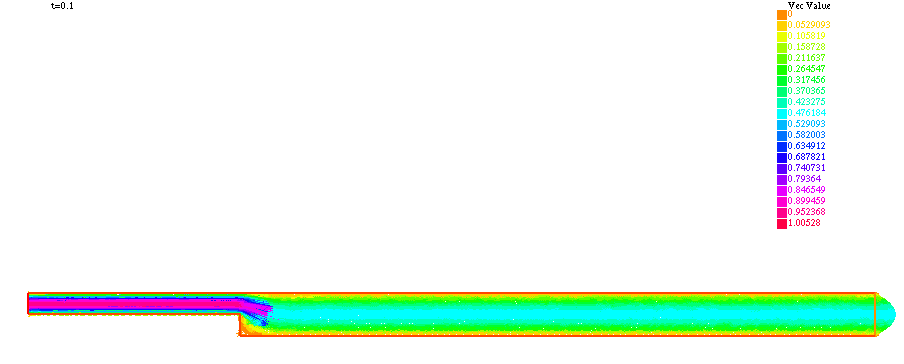
\includegraphics[width=0.49\linewidth]{image/ff++_NS_nu=1_t=1_u.png}
	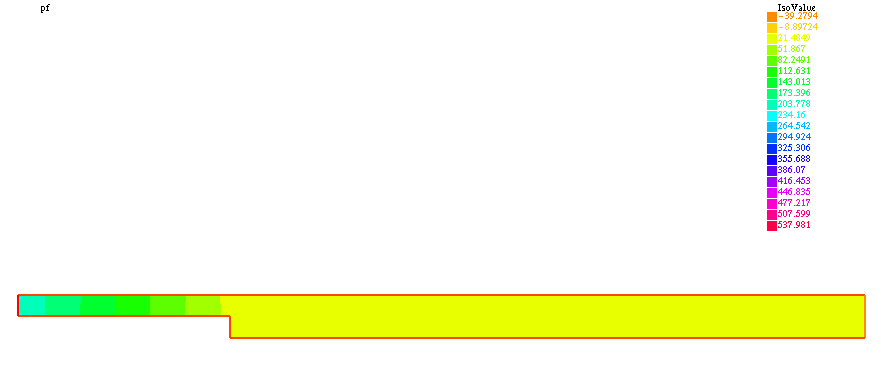
\includegraphics[width=0.49\linewidth]{image/c++_NS_nu=1_t=1_p.png}
	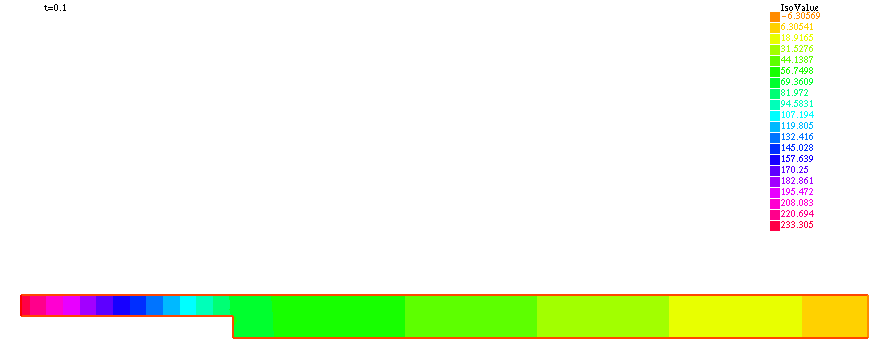
\includegraphics[width=0.49\linewidth]{image/ff++_NS_nu=1_t=1_p.png}
\end{figure}

\begin{figure}[!t]
	\caption{Vitesse et pression $\nu = 1,t=0.2$, C++ VS FF++}
	\centering
	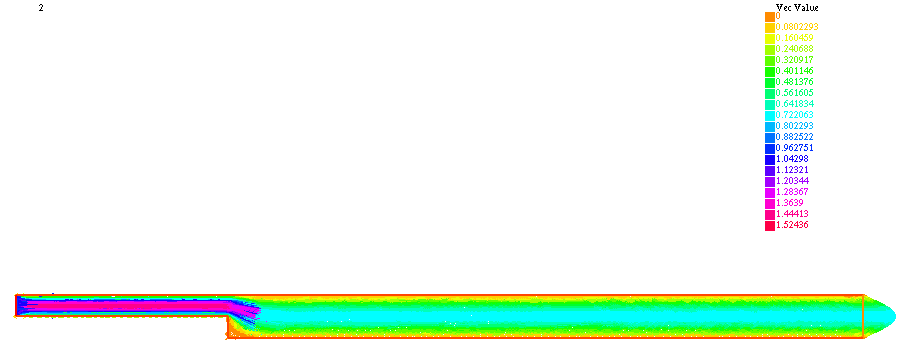
\includegraphics[width=0.49\linewidth]{image/c++_NS_nu=1_t=2_u.png}
	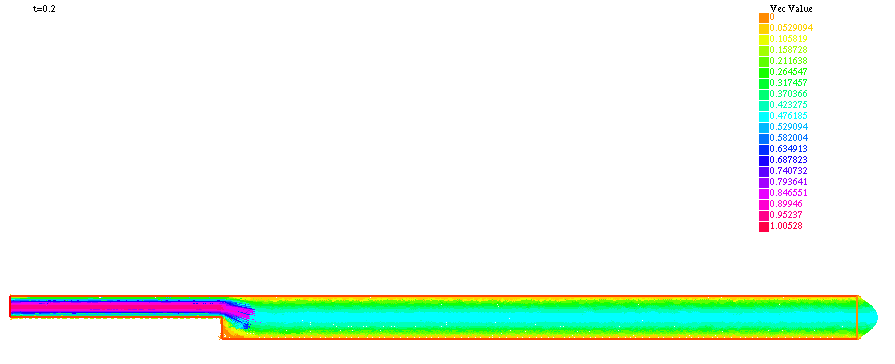
\includegraphics[width=0.49\linewidth]{image/ff++_NS_nu=1_t=2_u.png}
	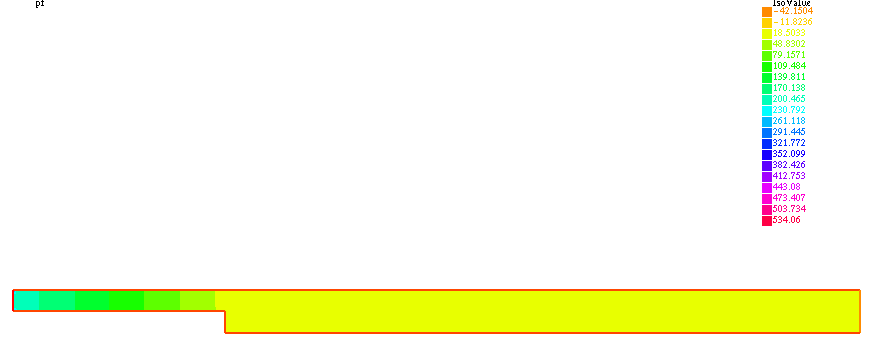
\includegraphics[width=0.49\linewidth]{image/c++_NS_nu=1_t=2_p.png}
	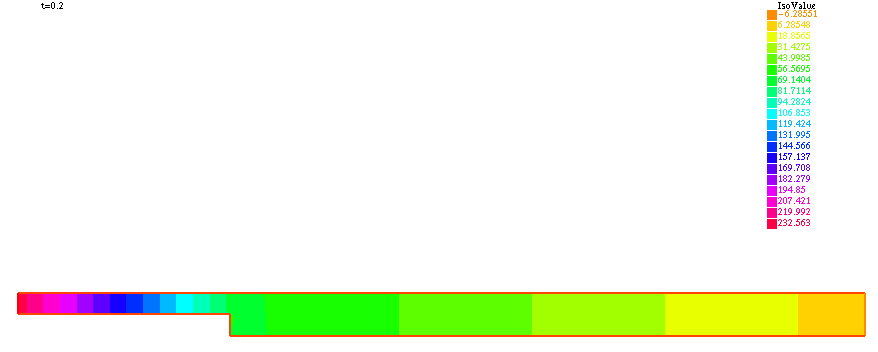
\includegraphics[width=0.49\linewidth]{image/ff++_NS_nu=1_t=2_p.png}
\end{figure}

On notera également que les temps d’exécution ne sont pas les mêmes, FF++ est plus rapide que le code C++. Cela est principalement dû à la fonction qui calcule le second membre pour Navier-Stokes qui n'est pas optimale et qui a sûrement encore quelques bugs de calcul.

\subsection{Le cas qui fonctionne moins bien}

En effet, si on diminue la viscosité à $\nu = 0.1$, on obtient déjà des solutions qui diffèrent de beaucoup après quelques pas de temps à celles de FF++. Voici les graphs :

\begin{figure}[!h]
	\caption{Vitesse et pression $\nu = 0.1,t=0$, C++ VS FF++}
	\centering
	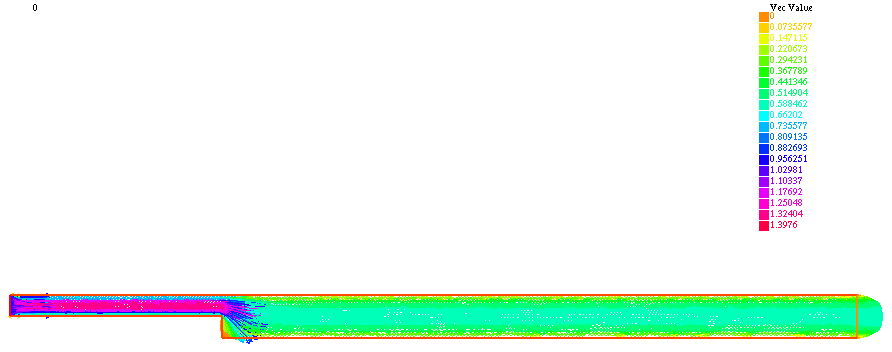
\includegraphics[width=0.49\linewidth]{image/c++_NS_nu=01_t=0_u.png}
	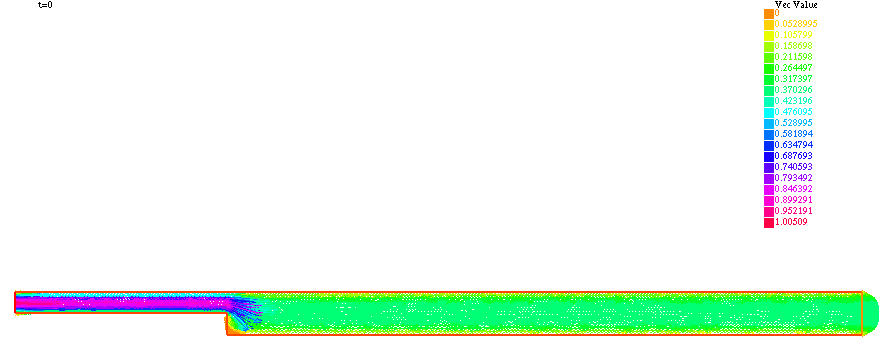
\includegraphics[width=0.49\linewidth]{image/ff++_NS_nu=01_t=0_u.png}
	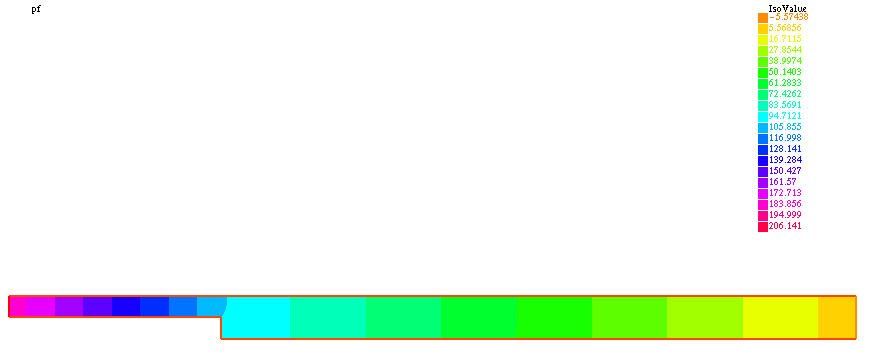
\includegraphics[width=0.49\linewidth]{image/c++_NS_nu=01_t=0_p.png}
	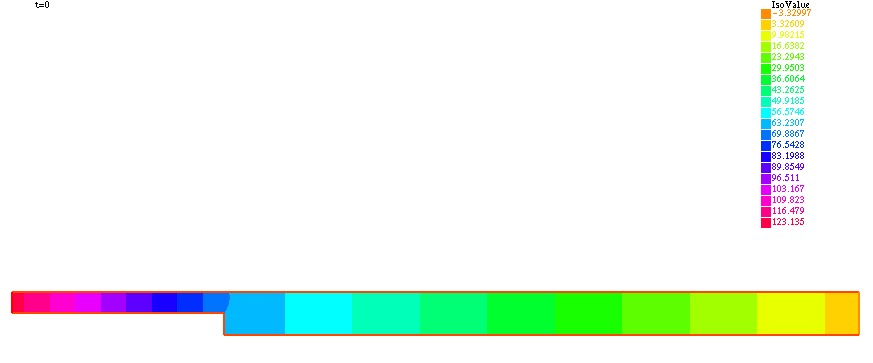
\includegraphics[width=0.49\linewidth]{image/ff++_NS_nu=01_t=0_p.png}
\end{figure}

\begin{figure}[!h]
	\caption{Vitesse et pression $\nu = 0.1,t=0.3$, C++ VS FF++}
	\centering
	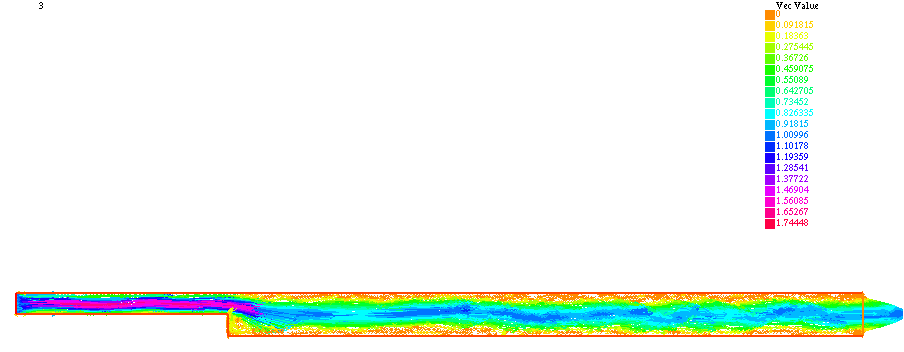
\includegraphics[width=0.49\linewidth]{image/c++_NS_nu=01_t=3_u.png}
	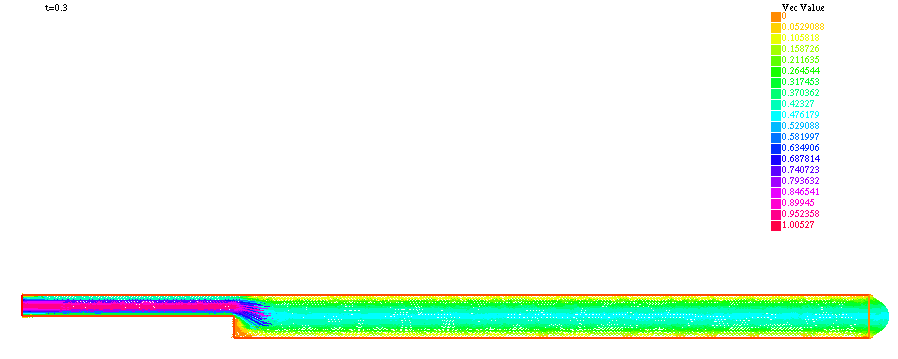
\includegraphics[width=0.49\linewidth]{image/ff++_NS_nu=01_t=3_u.png}
	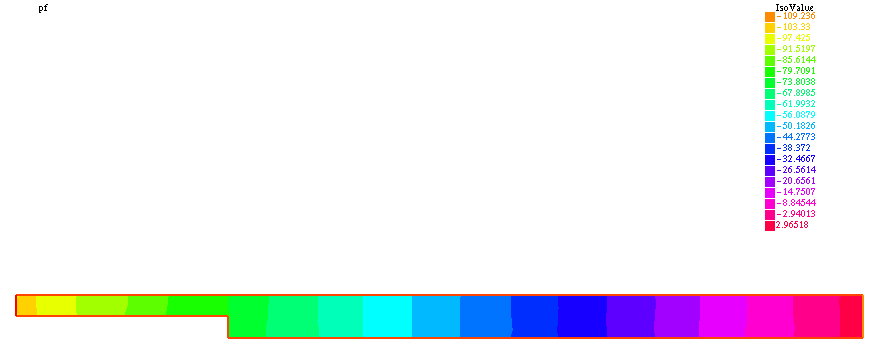
\includegraphics[width=0.49\linewidth]{image/c++_NS_nu=01_t=3_p.png}
	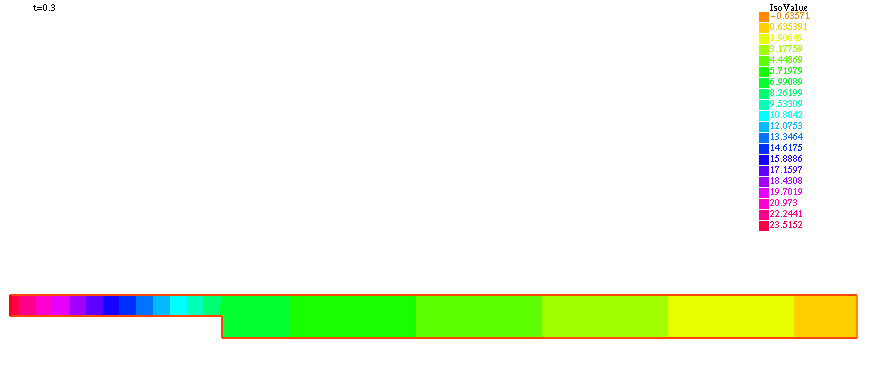
\includegraphics[width=0.49\linewidth]{image/ff++_NS_nu=01_t=3_p.png}
\end{figure}

\begin{figure}[!t]
	\caption{Vitesse et pression $\nu = 0.1,t=0.6$, C++ VS FF++}
	\centering
	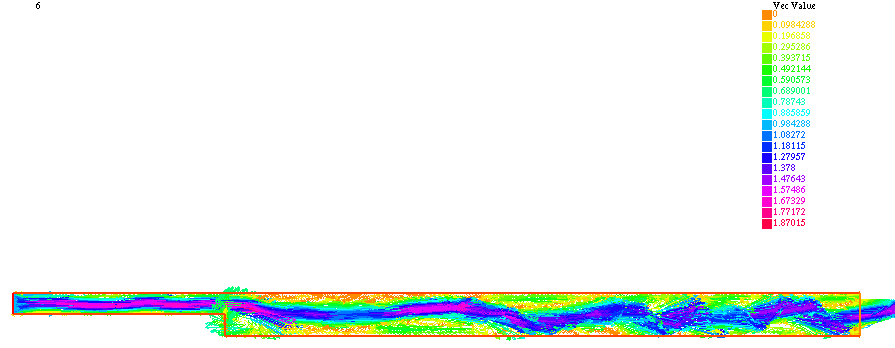
\includegraphics[width=0.49\linewidth]{image/c++_NS_nu=01_t=6_u.png}
	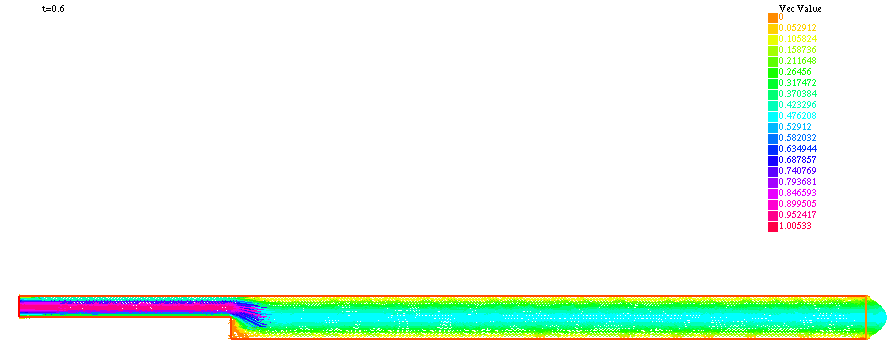
\includegraphics[width=0.49\linewidth]{image/ff++_NS_nu=01_t=6_u.png}
	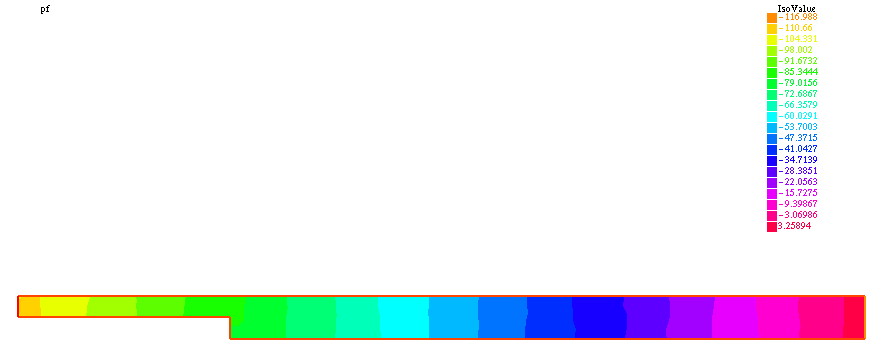
\includegraphics[width=0.49\linewidth]{image/c++_NS_nu=01_t=6_p.png}
	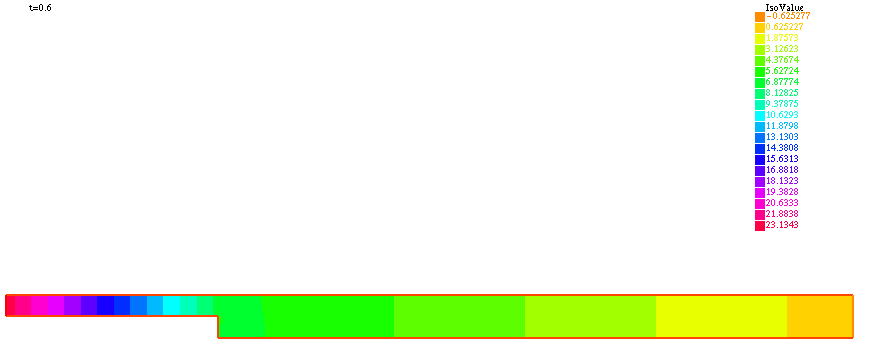
\includegraphics[width=0.49\linewidth]{image/ff++_NS_nu=01_t=6_p.png}
\end{figure}

\newpage

\textbf{Réferences}

[1] Mathematical Aspects of Discontinuous Galerkin Methods, de A. Ern et D. A. Di Pietro

[2] Finite Element Methods for Navier-Stokes Equations, V. Girault
et P.-A. Raviart

[3] Une méthode des caractéristiques d’ordre deux sur maillages mobiles pour la résolution des équations de Navier-Stokes incompressible par éléments, de Gilles Fourestey


\end{document}

